\documentclass[11pt]{article}
\usepackage[a4paper,margin=25mm,headheight=14pt]{geometry}
\usepackage[T1]{fontenc}
\usepackage{lmodern}
\usepackage{amsmath,amssymb,amsthm,mathtools}
\usepackage{microtype,booktabs,array,graphicx,xcolor}
\usepackage{enumitem,fancyhdr,xurl}
\usepackage[colorlinks=true,linkcolor=blue!45!black,citecolor=blue!45!black,urlcolor=blue!45!black]{hyperref}
\hypersetup{pdftitle={Finite observations of arithmetic Levy paths and critical recovery of symplectic forms},pdfauthor={Research note prepared for Vladimir Reshetnikov}}
\newtheorem{theorem}{Theorem}[section]
\newtheorem{lemma}[theorem]{Lemma}
\newtheorem{proposition}[theorem]{Proposition}
\newtheorem{corollary}[theorem]{Corollary}
\theoremstyle{remark}
\newtheorem{remark}[theorem]{Remark}
\numberwithin{equation}{section}
\setlist{topsep=4pt,itemsep=3pt}
\setlength{\emergencystretch}{2em}
\pagestyle{fancy}
\fancyhf{}
\fancyhead[L]{\small Finite observation and critical recovery}
\fancyhead[R]{\small ProveIt research extensions}
\fancyfoot[C]{\thepage}
\renewcommand{\headrulewidth}{0.3pt}
\title{\textbf{Finite observations of arithmetic L\'evy paths\\and critical recovery of symplectic forms}\\[0.7em]
\large Two extensions of the ProveIt GRH programme}
\author{Research note prepared for Vladimir Reshetnikov}
\date{27 November 2026}
\begin{document}
\maketitle
\begin{abstract}
We develop two further results from the analytic and finite-algebraic parts of the ProveIt generalized Riemann hypothesis programme. First, a fixed interval of a Dirichlet Li--L\'evy process suffices to recover any fixed finite set of real prime character values from progressively finer, noisy position observations. The noise may be chosen after the path is observed. We give an explicit estimator, mean-square bounds, a joint Gaussian limit, a finite-sample bound with specified constants, and a finite-family character decoder. Every known error bound tending to zero is admissible, with a suitable bandwidth. Fixed-order extrapolation yields achieved mesh exponents approaching one quarter.

Second, we prove critical-window nullity universality for random decomposable bivectors, both without a constraint and within the hyperplane defined by a hidden symplectic form. At $\binom n2-1+a$ observations the limiting laws are explicit rectangular finite-field matrix laws, with an exponential-in-$n$ error bound. This gives exact limiting linear-recovery probabilities, optimal tests based on solution-space dimension, and the complete limiting distribution of the extra observations needed for a unique linear solution. Over $\mathbb F_2$ the mean extra cost tends to $1.6066951524$.

The analytic result uses the repository's Dirichlet-GRH input; the finite-field result is unconditional. Both have complete mathematical proofs here. Neither new proof has been formalized in Lean. Their relation to earlier reports and classical probability and coding-theory methods is stated explicitly.
\end{abstract}
\tableofcontents
\newpage
\section{Source analysis and the new contributions}

\subsection{The pinned source and its mathematical scope}

The source is Vladimir Reshetnikov's ProveIt repository. We use its directory
\path{Analysis/GeneralizedRiemannHypothesis}, at commit
\begin{center}
\small\texttt{7c24c5481fc0c8101b22b7e7cfab8321921c0faa}.
\end{center}
Its current article merges 194 earlier reports into 20 subject sections; its catalogue lists 1,200 theorem-like results. The README describes this as a merger of reports, without recomputing their mathematics. Our analysis used the current catalogue and source modules, followed by detailed examination of the parts relevant to these two extensions. Thirty-nine retrieved source files were checked against their pinned Git blob hashes. The accompanying provenance file records the inspected source set~\cite{ProveIt2026}.

The upstream result used by the article is RH and GRH for Dirichlet $L$-functions, at revision \texttt{72fead102f663d5c7a407964a13dc0cf9d977207} of \texttt{lsernau/grh-lean}. The exported statements use Mathlib's zeta and Dirichlet $L$-functions. Sutherland's verification page reports successful independent kernel and external-checker runs for this revision~\cite{Sutherland2026}. We did not replay that large verification. The first result below takes the source's Dirichlet-GRH theorem as input, and the second needs only finite linear algebra and probability.

The underlying research programme has two useful interfaces. On the analytic side, zero-location and explicit formulas convert oscillatory sums over zeros into prime-power coefficients. On the arithmetic and algebraic side, the source proof uses finite spanning estimates, tight frames, and Fourier estimates for matrix observations. The present extensions use these two interfaces separately. They do not transfer the zero-location theorem to another family of $L$-functions.

\subsection{First contribution: a quantitative finite-observation theorem}

The article's \texttt{li:thm:decoder} recovers $\Re\chi(p)$ from exact jumps of the Li--L\'evy process. Its \texttt{li:thm:grid} shows that every fixed finite grid has mutually absolutely continuous laws across characters. Question \texttt{li:q:paths} asks about discrete noisy observations. We answer its fixed-family, fixed-duration part.

For mesh $h$, increment-error bound $\eta$, and spectral bandwidth $T$, Theorem~\ref{thm:noisy-grid} constructs an estimator from positions alone with root-mean-square error bounded by
\begin{equation}\label{overview:basic}
C\left(\sqrt{\frac{\log T}{T}}
 +\frac{\log^2T}{T}+hT^3\log^2T+\eta T^2\log T\right)
\end{equation}
for fixed observation duration and sufficiently large $T$. The bound follows from the proof and the variance estimate in Theorem~\ref{thm:extrapolation}, with $m=1$. The error may be adversarial; there is no assumption of independent or mean-zero observation noise.

The conservative choice $T=\min(h^{-1/4},\eta^{-1/3})$ works for any $h\to0$ and $\eta\to0$, and also preserves the exact-jump Gaussian limiting covariance after multiplication by the window factor $\int w^2$. Thus one short interval contains enough arithmetic information for consistent finite-family identification even under vanishing measurement error. This is compatible with the impossibility of zero-error identification from one fixed finite grid.

Higher-order correction gives the achieved bound
\begin{equation}\label{overview:rates}
\operatorname{RMSE}\ \le C_m\max\left\{
h^{m/(4m+3)}\bigl(\log(1/h)\bigr)^{(3m+2)/(4m+3)},\quad
\eta^{1/5}\bigl(\log(1/\eta)\bigr)^{3/5}\right\}.
\end{equation}
Here $m$ is fixed, the second term is omitted for $\eta=0$, and $C_m$ also depends on the fixed arithmetic data. The mesh exponent approaches $1/4$ as the fixed order is increased. These are constructive upper bounds, not minimax claims. The conductor-uniform and optimal-information portions of the article's open question remain unresolved.

\subsection{Second contribution: the complete linear critical window}

An earlier delivered note, \emph{Recovering a Hidden Symplectic Form}, showed that $d=\binom n2-1$ is the threshold for recovering a hidden nondegenerate alternating form from random two-planes on which it vanishes. It proved success and failure across diverging additive windows, and a critical second-moment estimate. It did not determine the critical nullity distribution. This earlier note was inspected in its supplied working copy, with its hash recorded in the provenance file; it is more recent than the relevant merged article text.

The new Theorem~\ref{crit:main} gives the entire fixed-offset nullity law, with an explicit finite error bound. Its most direct consequence is
\[
\Pr\{N_{d+a}=\langle H\rangle\}
\longrightarrow \prod_{j=a+1}^{\infty}(1-q^{-j})
\qquad(t=d+a,\ a\ge0).
\]
Here $N_t$ is the space of forms satisfying the observed linear equations, so the event means that the hidden form is their only solution up to scale. For $a<0$ linear uniqueness is impossible. The result applies in every characteristic and uniformly in the hidden form. It also determines the optimal limiting test that retains only the solution-space dimension, and the distribution and all moments of the observation overhead.

The delicate point is universality. Each observation is a decomposable bivector and its coordinates are strongly dependent; in the planted experiment it lies in a prescribed symplectic hyperplane. The iid matrix law cannot simply be assumed. We prove that after an initial part of the sample has excluded forms of low rank, every subsequent decrease of the solution-space dimension has essentially the same probability as for a uniform random linear equation. The resulting coupling controls the whole final dimension process.

\subsection{Relation to prior work and the scope of novelty}

Small-time L\'evy moment expansions, high-frequency estimation, jump recovery, and Richardson extrapolation are established methods~\cite{Figueroa2008,Nickl2016,Gonzalez2021}. The arithmetic content here is the moving prime-frequency probe, its explicit sensitivity to noise, and its combination with a fixed observation horizon and a singular atomic zero measure. We give the required bounds for that setting rather than assuming that a fixed-test-function theorem covers it.

The rectangular iid nullity law is classical; Fulman and Goldstein give sharp total-variation results~\cite{FulmanGoldstein2015}. Low-rank counting and high-rank near-uniformity also appear in work on squares of random linear codes and products of codes~\cite{Cascudo2015,Randriambololona2015}. Cascudo and coauthors prove threshold and critical first-moment statements for quadratic evaluations. Their sampling model is different, and the inspected paper does not supply the fixed-offset planted symplectic nullity law proved here. The new finite-field content is the structured-row universality theorem and its explicit recovery, testing, and stopping-time consequences.

These are proved extensions beyond the inspected source statements and the preceding hidden-form note. The literature search establishes relevant antecedents and a scoped comparison; it does not certify worldwide publication priority. The report makes no claim that the new theorems have been independently peer reviewed or formally verified.

\begin{center}
\small
\begin{tabular}{@{}>{\raggedright\arraybackslash}p{.22\linewidth}>{\raggedright\arraybackslash}p{.34\linewidth}>{\raggedright\arraybackslash}p{.35\linewidth}@{}}
\toprule
Direction & Earlier result & Extension proved here\\
\midrule
Arithmetic paths & Exact jump decoder; overlapping fixed-grid laws & Noisy position estimator, fixed-horizon consistency, CLT and achieved mesh--precision rates\\[4pt]
Hidden symplectic form & Threshold across diverging sample gaps & Full fixed-offset nullity law; exact linear-recovery and dimension-test curves; stopping-time moments\\
\bottomrule
\end{tabular}
\end{center}

% Mathematical fragment. Requires amsmath, amssymb, amsthm and theorem environments.
% All constants below are fixed-character constants unless explicitly stated otherwise.

\section{Recovering a character from finitely many noisy positions}
\label{sec:noisy-grids}

The starting point is the symmetric Li--L\'evy process in the repository's
\path{Article/sections/li.tex}. Its exact-path decoder uses individual jumps
in progressively smaller size bands.  The theorem below replaces those jumps
by increments between finitely many observed positions.  It permits bounded
errors chosen after the entire path is seen.  The observation duration remains
fixed.  In particular, increasing the duration is not needed for consistency.

The arithmetic inputs are the signed zero-counting formula and the rational
prime-frequency formula proved in the repository, labels
\texttt{li:lem:bands} and \texttt{zer:lem:rational}.  Their application to the
Li coefficients uses the upstream Dirichlet-GRH theorem.  No simplicity,
spacing, linear independence, or disjointness assumption on zero ordinates is
made.  The probabilistic arguments below are independent of any formal
verification status of the upstream implementation.

\subsection{The process and an explicit estimator}

Let $\chi$ be a primitive Dirichlet character; the conductor-one character
represents $\zeta$.  Count all signed ordinates $\gamma$ of its nontrivial
zeros, including multiplicities.  Put
\[
 \theta(\gamma)=2\arctan\frac1{2\gamma}\quad(\gamma\ne0),\qquad
 \theta(0)=\pi,\qquad
 \nu_\chi=\frac12\sum_\gamma
       (\delta_{\theta(\gamma)}+\delta_{-\theta(\gamma)}).
\]
Thus a central zero of multiplicity $m$ contributes $m/2$ at each of
$\pi$ and $-\pi$.  Let $X=X^\chi$ be the real, symmetric, compensated
L\'evy process with no Gaussian component and
\[
 \mathbb E_\chi e^{iuX_s}
 =\exp\left[-s\int(1-\cos uy)\,\nu_\chi(dy)\right].
\]
Its small jumps have infinite total variation.  Their squared sizes are
integrable: $\int y^2\nu_\chi(dy)<\infty$.  The compensation is therefore
part of the definition.

Choose once and for all $w\in C_c^\infty(\mathbb R)$ supported on $[1,2]$,
$w\ge0$, with
$\int_1^2 w(v)\,dv=1$, and write $J_w=\int_1^2w(v)^2\,dv$.
For $0<|y|<\pi$ put
\[
 G(y)=\frac1{2\tan(|y|/2)},\qquad
 a_p=\frac{\pi\sqrt p}{\log p},\qquad
 f_{T,p}(y)=w\!\left(\frac{G(y)}T\right)
                    \cos(G(y)\log p),                         \tag{NG1}
\]
and set $f_{T,p}=0$ elsewhere.  Here $p$ is a prime and $T\ge2$ is a
chosen spectral height.  The compact support of $w$ makes $f_{T,p}$ smooth
on the whole real line.  A concrete alternative requiring only $C^4$
regularity for the first-order theorem is
\[
 w(v)=2772(v-1)^5(2-v)^5\mathbf1_{[1,2]}(v),\qquad
 J_w=2772^2\frac{(10!)^2}{21!}.                         \tag{NG2}
\]
Its derivatives through order four vanish at both endpoints.  For the
arbitrary-order construction later, use $C^\infty$ or the analogous
beta window with exponent at least $2m+3$ for correction order $m$.

Fix $t>0$.  At mesh $h=t/n$ observe positions $Y_0,\ldots,Y_n$ satisfying
\[
 \left|(Y_j-Y_{j-1})-(X_{jh}-X_{(j-1)h})\right|\le\eta
 \quad(1\le j\le n).                                      \tag{NG3}
\]
The errors can be random, dependent, or selected adversarially from the
whole path.  For example, position errors $|Y_j-X_{jh}|\le\varepsilon$
give (NG3) with $\eta=2\varepsilon$.  Define
\[
 \widehat D_{T,h,t}(p)
   =-\frac{a_p}{tT}\sum_{j=1}^n f_{T,p}(Y_j-Y_{j-1}),\qquad
 D^0_{T,h,t}(p)
   =-\frac{a_p}{tT}\sum_{j=1}^n f_{T,p}(X_{jh}-X_{(j-1)h}).   \tag{NG4}
\]
The estimator needs no conductor, zero table, zero multiplicities, or
candidate character.  It uses $n$ elementary evaluations per probe prime.
If each computed probe value has an additional absolute evaluation error
at most $\xi$, its effect on (NG4) is at most $a_p\xi/(hT)$.
Thus certified evaluation precision can be selected separately from the
observation-error bound; floating-point demonstrations are not an
automatic certificate at arbitrarily large $T$.

\begin{theorem}[Noisy finite-grid arithmetic recovery]
\label{thm:noisy-grid}
Fix $\chi$, $t>0$, $w$, and distinct primes $p_1,\ldots,p_k$.  All asymptotic
constants in this theorem may depend on these fixed choices.  Let
$h=t/n\to0$, $T\to\infty$, and suppose (NG3) holds.
\begin{enumerate}
\item The clean estimator has mean
\[
 \mathbb E_\chi D^0_{T,h,t}(p)
 =\Re\chi(p)+O\!\left(\frac{\log^2T}{T}
                          +hT^3\log^2T\right).               \tag{NG5}
\]
Whenever $hT^3\log^2T\le1$, its covariances satisfy
\[
 \operatorname{Cov}_\chi(D^0(p),D^0(r))
 =\mathbf1_{p=r}\frac{\pi pJ_w}{2t(\log p)^2}
                    \frac{\log T}{T}
  +O\!\left(\frac1{tT}+\frac{hT^2\log^2T}{t}\right).        \tag{NG6}
\]
\item Uniformly over every perturbation satisfying (NG3), if
$\eta\le1/(16T)$ then
\[
 \|\widehat D(p)-D^0(p)\|_{L^2}
 \le C\eta\left(T^2\log T+
                 T^{3/2}\sqrt{\frac{\log T}{t}}\right).     \tag{NG7}
\]
In particular, if
\[
 hT^3\log^2T\longrightarrow0,
 \qquad \eta T^2\log T\longrightarrow0,                     \tag{NG8}
\]
then all $\widehat D(p_j)\to\Re\chi(p_j)$ in mean square.
\item If the stronger conditions
\[
 hT^{7/2}(\log T)^{3/2}\longrightarrow0,
 \qquad \eta T^{5/2}\sqrt{\log T}\longrightarrow0            \tag{NG9}
\]
hold, then
\[
 \sqrt{\frac{tT}{\log T}}
 \bigl(\widehat D(p_j)-\Re\chi(p_j)\bigr)_{j=1}^k
 \quad\Longrightarrow\quad
 N_k\!\left(0,
  \operatorname{diag}_{j\le k}
       \frac{\pi p_jJ_w}{2(\log p_j)^2}\right).              \tag{NG10}
\]
Thus the limiting errors at distinct probe primes are independent.
\end{enumerate}
\end{theorem}

\begin{corollary}[Any vanishing error bound suffices]
\label{cor:any-noise}
For any $h\to0$ and any known $\eta\to0$, choose
\[
 T=\min\{h^{-1/4},\eta^{-1/3}\},                            \tag{NG11}
\]
where $\eta^{-1/3}=+\infty$ if $\eta=0$.  Then (NG9) holds and the
conclusions of the theorem follow.  There is no required relative rate
between the two vanishing quantities $h$ and $\eta$.
\end{corollary}

\begin{proof}
For large $n$, $T\to\infty$.  Since $T\le h^{-1/4}$,
$hT^{7/2}(\log T)^{3/2}\le
C h^{1/8}(\log(1/h))^{3/2}\to0$.
When $\eta>0$, the other inequality gives
$\eta T^{5/2}\sqrt{\log T}
\le C\eta^{1/6}\sqrt{\log(1/\eta)}\to0$.
\end{proof}

The result is consistent with the repository's finite-grid equivalence
theorem: every \emph{fixed} finite grid has overlapping statistical laws.
Here the number of samples tends to infinity, and the error probability
tends to zero.  No fixed finite grid is asserted to identify the character
with probability one.

\subsection{The two analytic estimates}

\begin{lemma}[Weighted arithmetic moments]
\label{lem:weighted-moments}
For fixed primes $p,r$, as $T\to\infty$,
\begin{align*}
 I_p(T):=\int f_{T,p}\,d\nu_\chi
   &=-\frac{T}{a_p}\Re\chi(p)+O(\log^2T),\\
 I_{pp}(T):=\int f_{T,p}^2\,d\nu_\chi
   &=\frac{T\log T}{2\pi}J_w+O(T),\\
 I_{pr}(T):=\int f_{T,p}f_{T,r}\,d\nu_\chi
   &=O(\log^2T)\qquad(p\ne r).                            \tag{NG12}
\end{align*}
Also, for $0<u\le1$,
\[
 \nu_\chi(|y|>u)\le C u^{-1}\log(2/u),\qquad
 \int_{|y|\le u}y^2\nu_\chi(dy)\le C u\log(2/u).           \tag{NG13}
\]
\end{lemma}

\begin{proof}
The signed zero count is
$N_\chi(v)=\frac v\pi\log v+C_\chi v+O_\chi(\log(v+2))$.
Since $G(\theta(\gamma))=|\gamma|$, the zero count and partial summation
give
\[
 \int w(G/T)^2\,d\nu_\chi
       =\frac{T\log T}\pi J_w+O(T).
\]
The rational prime-frequency formula in the repository gives, for each
fixed rational $x>1$ and $T\le v\le2T$,
\[
 \sum_{T<|\gamma|\le v}\cos(\gamma\log x)
 =-\frac{(v-T)\Lambda(x)\Re\chi(x)}{\pi\sqrt x}
       +O_{\chi,x}(\log^2T),                              \tag{NG14}
\]
where the sum includes multiplicity; the main term is zero unless $x$ is
an integral prime power.  Stieltjes integration by parts against $w(v/T)$
gives the first formula in (NG12), because $\int w=1$ and
$\int|w'|<\infty$.  Apply the same argument with $w^2$ and use
$\cos^2 z=(1+\cos2z)/2$ for the second formula.
For distinct primes, product-to-sum leaves frequencies $\log(pr)$ and
$|\log(p/r)|$; neither argument is an integral prime power, proving the
third.  Finally $\theta(\gamma)\asymp1/|\gamma|$ for large ordinates gives
the first bound in (NG13).  Integration of $2v\nu_\chi(|y|>v)$ from $0$
to $u$ gives the second.  Finite large atoms and central zeros are absorbed
in the constant.
\end{proof}

\begin{lemma}[A generator bound for moving probes]
\label{lem:generator}
Let $L$ be the generator of $X$, so
\[
 Lg(x)=\frac12\int
       [g(x+y)+g(x-y)-2g(x)]\,\nu_\chi(dy).                \tag{NG15}
\]
For every integer $r\ge1$, if a bounded smooth function $g$ satisfies
$\|g^{(j)}\|_\infty\le M A^j$ for $0\le j\le2r$, $A\ge2$, then
\[
 \|L^r g\|_\infty\le C_r M[A\log(2A)]^r.                \tag{NG16}
\]
For fixed $p,w,r$, both $f_{T,p}$ and any fixed finite product of such
probes satisfy the derivative hypothesis with $A=T^2$ and constant $M$.
Consequently,
\[
 \|L^r f_{T,p}\|_\infty\ll T^{2r}(\log T)^r.             \tag{NG17}
\]
\end{lemma}

\begin{proof}
Write $\Delta_y g(x)=g(x+y)+g(x-y)-2g(x)$.  For a set of $r$ increments,
apply the integral second-derivative representation to those $y_i$ with
$A|y_i|\le1$, and the bound $\|\Delta_y\|\le4$ to all the others.
Commutation of differences and derivatives gives
\[
 \|\Delta_{y_1}\cdots\Delta_{y_r}g\|_\infty
 \le4^r M\prod_{i=1}^r\min\{1,A^2y_i^2\}.
\]
By (NG13),
\[
 B(A):=\int\min\{1,A^2y^2\}\,\nu_\chi(dy)
 \le\nu_\chi(|y|>A^{-1})+
      A^2\int_{|y|\le A^{-1}}y^2\nu_\chi(dy)
 \ll A\log(2A).
\]
The repeated integral is absolutely convergent, proving (NG16).
On the support of $f_{T,p}$, $|y|\asymp T^{-1}$ and
$|G^{(j)}(y)|\ll_j T^{j+1}$.  Differentiating (NG1) therefore gives
$\|f_{T,p}^{(j)}\|_\infty\ll_{j,p,w}T^{2j}$.  All endpoint
derivatives match zero because the window is smooth.  Leibniz' rule treats
products.
\end{proof}

\subsection{Proof of the noisy-grid theorem}

Let $P_sg(x)=\mathbb E g(x+X_s)$.  Twice applying the semigroup fundamental
theorem gives
\[
 P_hg(0)=g(0)+hLg(0)+\int_0^h(h-s)P_sL^2g(0)\,ds.       \tag{NG18}
\]
For the smooth compact probes this identity follows directly first with
the L\'evy measure truncated away from zero; the bounds in
Lemma~\ref{lem:generator} justify passage to the limit.  In particular,
no density for the atomic measure $\nu_\chi$ is required.
Since $f_{T,p}$ vanishes in a neighbourhood of zero, $f_{T,p}(0)=0$ and
$Lf_{T,p}(0)=I_p(T)$.  The semigroup is a contraction, and (NG17) yields
\[
 \mathbb E f_{T,p}(X_h)
       =hI_p(T)+O(h^2T^4\log^2T).                        \tag{NG19}
\]
Multiplying by $-a_p n/(tT)$ proves (NG5).  Apply the same calculation to
$f_{T,p}f_{T,r}$ and use independent stationary increments.  Under
$hT^3\log^2T\le1$, (NG19) is $O(hT)$, so subtracting the product of the
means contributes $O(h/t)$ to the covariance of the estimators.
Equations (NG12) and (NG19) now give (NG6).

For the noise estimate put $r_T=1/(8T)$ and
\[
 N_T=\#\{j:|X_{jh}-X_{(j-1)h}|\ge r_T\}.
\]
The support of $f_{T,p}$ lies in $|y|\ge\theta(2T)\ge1/(4T)$.
If $\eta\le1/(16T)$ and the two evaluations of a probe at a clean and
perturbed increment differ, the clean increment therefore has magnitude
at least $r_T$.  The mean value theorem gives the pathwise bound
\[
 |\widehat D(p)-D^0(p)|
 \le\frac{a_p\eta\|f'_{T,p}\|_\infty}{tT}N_T
 \le\frac{C\eta T}{t}N_T.                                \tag{NG20}
\]
Split $X_h$ into jumps larger than $r/2$ and its compensated symmetric
small-jump part.  The former occurs with probability at most
$h\nu_\chi(|y|>r/2)$, while the latter has variance
$h\int_{|y|\le r/2}y^2\nu_\chi(dy)$.  Thus
\[
 \mathbb P(|X_h|\ge r)
 \le h\left(\nu_\chi(|y|>r/2)+
             r^{-2}\int_{|y|\le r/2}y^2\nu_\chi(dy)\right).
                                                                  \tag{NG21}
\]
At $r=r_T$, the parenthesis is $O(T\log T)$ by (NG13).  The count $N_T$
is binomial, independently of how the perturbations are selected, with
\[
 \mathbb E N_T\le CtT\log T,\qquad
 \mathbb E N_T^2\le C(tT\log T)^2+CtT\log T.
\]
Together with (NG20), this proves (NG7).  Equations (NG5)--(NG7) prove
mean-square consistency under (NG8).

For the central limit theorem, take any fixed linear combination of the
clean coordinates.  After multiplication by $\sqrt{tT/\log T}$ its
centred summands are bounded by $C/\sqrt{tT\log T}\to0$.
Their total variance tends, by (NG6), to the corresponding quadratic form
of the diagonal matrix in (NG10), because (NG9) implies
$hT^3\log T\to0$.  The bounded triangular-array Lindeberg theorem and
Cram\'er--Wold give the centred joint Gaussian limit.  Multiplying (NG5)
by $\sqrt{tT/\log T}$ shows that its bias vanishes under (NG9).
Finally (NG7) gives a vanishing $L^2$ perturbation after the same
normalization; Slutsky's theorem proves (NG10), uniformly for all errors
obeying (NG3).

\subsection{A finite-sample bound with specified input constants}

The following bound keeps its constants visible. It becomes a numerical error certificate only after upper bounds for these model-dependent quantities have been supplied. Upper bounds for its
input quantities can be substituted throughout; in a fixed finite
character family they can be replaced by family-wide maxima.

\begin{proposition}[Confidence bound including adversarial error]
\label{prop:grid-confidence}
Fix one prime $p$, let $f=f_{T,p}$, and put
\begin{gather*}
 M=\|f\|_\infty,\quad L_T=\|f'\|_\infty,
 \quad K_1=\|L^2f\|_\infty,\quad K_2=\|L^2(f^2)\|_\infty,\\
 I_2=\int f^2\,d\nu_\chi,\quad
 b_{\rm ar}=\left|-\frac{a_p}T\int f\,d\nu_\chi-\Re\chi(p)\right|,\quad
 V=t(I_2+hK_2/2),\\
 \beta_T=\nu_\chi(|y|>r_T/2)+
         r_T^{-2}\int_{|y|\le r_T/2}y^2\nu_\chi(dy),
 \qquad \mu=t\beta_T.
\end{gather*}
If (NG3) holds with $\eta\le1/(16T)$, then, for every $u>0$, with
probability at least $1-3e^{-u}$,
\begin{align*}
 |\widehat D(p)-\Re\chi(p)|\le {}&b_{\rm ar}
              +\frac{a_phK_1}{2T}
              +\frac{a_p}{tT}
                     \left(\sqrt{2Vu}+\frac43Mu\right)\\
 &+\frac{a_p\eta L_T}{tT}
                     \left(\mu+\sqrt{2\mu u}+\frac23u\right).
                                                               \tag{NG22}
\end{align*}
The event on which this holds can be chosen independently of the
perturbations, so the statement is simultaneous over all admissible
perturbations of a realized clean grid.
\end{proposition}

\begin{proof}
By (NG18), the clean bias is at most the first two terms.  Its unnormalized
centred sum consists of independent variables bounded by $2M$, with total
variance at most $V$.  Bernstein's inequality bounds that sum in absolute
value by $\sqrt{2Vu}+4Mu/3$ outside an event of probability $2e^{-u}$.
The binomial count in (NG20) has mean at most $\mu$ by (NG21).
The one-sided Bernstein inequality gives
$N_T\le\mu+\sqrt{2\mu u}+2u/3$ outside an event of probability $e^{-u}$.
Use (NG20) and the union bound.
\end{proof}

\subsection{Recovering the whole arithmetic label}

\begin{theorem}[Identification in any fixed finite candidate family]
\label{thm:finite-family}
Let $\mathcal C$ be a finite set of primitive Dirichlet characters, with
one representative from each conjugacy orbit.  There are finitely many
primes $p_1,\ldots,p_k$ for which the codewords
\[
 c_\chi=(\Re\chi(p_1),\ldots,\Re\chi(p_k)),\qquad\chi\in\mathcal C,
\]
are distinct.  Write $\Delta=\min_{\chi\ne\psi}\|c_\chi-c_\psi\|_\infty>0$,
with the singleton family interpreted trivially.  The nearest-codeword
rule
\[
 \widehat\chi=\operatorname*{argmin}_{\psi\in\mathcal C}
          \max_{j\le k}|\widehat D(p_j)-\Re\psi(p_j)|       \tag{NG23}
\]
with any fixed tie rule satisfies
\[
 \sup_{\chi\in\mathcal C}\sup_{\text{errors satisfying (NG3)}}
        \mathbb P_\chi(\widehat\chi\ne\chi)\longrightarrow0
                                                               \tag{NG24}
\]
under (NG8).  For a quantitative bound, apply (NG22) at all the probe
primes and require each right-hand side to be less than $\Delta/2$;
the error probability is then at most $3ke^{-u}$.
In particular, for all sufficiently large $T$ along any sequence obeying
(NG8), there is a constant $c>0$ such that the same uniform error
probability is at most
\[
             3k\exp\!\left(-\frac{ctT}{\log T}\right).     \tag{NG24a}
\]
The constant and the threshold are permitted to depend on the fixed
candidate family, the window, the probe primes, and the fixed duration.
\end{theorem}

\begin{proof}
If two primitive characters have the same real values at every prime,
induce them to the unit group modulo the least common multiple of their
conductors.  Every reduced residue class contains a prime, so their sums
with their conjugates coincide as functions on this finite group.
Linear independence of group characters implies that they belong to the
same conjugacy orbit; primitive antecedents are unique.  For each of the
finitely many distinct pairs, select one distinguishing prime.  Their
union gives the required finite set.  If the maximum estimation error is
less than $\Delta/2$, the correct codeword is uniquely nearest.
Theorem~\ref{thm:noisy-grid}, a finite union bound, and then the maximum of
finitely many constants prove (NG24).
For the exponential conclusion use $u=ctT/\log T$ in (NG22).
Uniformly over the finite family, $V=O(tT\log T)$ and
$\mu=O(tT\log T)$. The stochastic square-root term is $O(\sqrt c)$,
its linear term is $O(c/\log T)$, and the noise term is
$O(\eta T^2\log T)$. Both bias terms tend to zero by (NG8).
Choose $c$ sufficiently small compared with $\Delta^2$, then take $T$
large and apply the finite union bound.
\end{proof}

In particular, this applies to the entire finite family of primitive
characters of conductor at most a prescribed $Q$.  The family, time
duration, and prime probes are fixed in the asymptotic statements.  This
does not assert statistical constants uniform in a growing conductor
bound.  It resolves the fixed-family noisy-grid part of the repository's
question \texttt{li:q:paths}; its requests for optimal information and
uniform conductor/duration/probe-prime complexity remain separate.

\subsection{Higher-order mesh correction and its cost}

The leading discretization error can be cancelled by the standard
Richardson extrapolation identity.  The variance bound needed for the
result below uses the support of the probes, rather than an unjustified
Gaussian approximation at the accelerated meshes.

\begin{theorem}[Arbitrary fixed-order correction]
\label{thm:extrapolation}
Fix an integer $m\ge1$ and positive numbers $\alpha_1,\ldots,\alpha_m$
with $\sum\alpha_j=1$.  Split the observed interval into consecutive
disjoint blocks whose endpoints lie on the base grid, with lengths tending to $\alpha_jt$. In block $j$, use
nonoverlapping increments of length $jh$, discarding at most $jh$ at its
end, and normalize its estimator (NG4) by its actual used duration $t_j$.
Assume that the error in every used increment is at most $\eta$.
Set
\[
 b_j=(-1)^{j+1}\binom mj,\qquad
 \widehat D^{[m]}(p)=\sum_{j=1}^m b_j\widehat D_j(p).       \tag{NG25}
\]
For fixed $m,\chi,p,w,t,\alpha$, and $\eta\le1/(16T)$,
\begin{align*}
 \|\widehat D^{[m]}(p)-\Re\chi(p)\|_{L^2}
 \le C\bigg(&\sqrt{\frac{\log T}{T}}
          +\frac{\log^2T}{T}
          +h^mT^{2m+1}(\log T)^{m+1}
          +\eta T^2\log T\bigg).                         \tag{NG26}
\end{align*}
If the supplied data are noisy \emph{positions} with individual errors
bounded by $\varepsilon$, the hypothesis holds with $\eta=2\varepsilon$
for all the coarser increments as well.  If only elementary increment
errors are bounded by $\eta_0$, use $\eta=m\eta_0$ instead.
\end{theorem}

\begin{proof}
Repeated semigroup integration, justified by Lemma~\ref{lem:generator},
gives
\[
 \frac1s\mathbb E f_{T,p}(X_s)
 =\sum_{r=1}^m\frac{s^{r-1}}{r!}(L^rf_{T,p})(0)
       +O\bigl(s^mT^{2m+2}(\log T)^{m+1}\bigr).           \tag{NG27}
\]
The finite-difference identities
$\sum_{j=1}^m b_j=1$ and
$\sum_{j=1}^m b_jj^r=0$ for $1\le r<m$ cancel all the displayed
discretization terms except $Lf(0)=I_p(T)$.  Dividing by $T$ proves the
bias part of (NG26).

For variance, $|f_{T,p}(x)|\le M\mathbf1_{\{|x|\ge r_T\}}$ and (NG21)
give, for \emph{every} $s>0$,
\[
 \mathbb E f_{T,p}(X_s)^2\le M^2s\beta_T
                         \ll sT\log T.
\]
The variance of the normalized clean block estimator is therefore at
most $C\log T/(t_jT)$.  The disjoint blocks have independent increments,
so the variance of their weighted sum is at most
$C(\sum b_j^2/\alpha_j)\log T/(tT)$ for large $n$.
The pathwise perturbation argument (NG20), applied in each block and
then combined by the triangle inequality in $L^2$, proves the noise term.
Since $t,m,\alpha$ are fixed, its lower-order term
$\eta T^{3/2}\sqrt{\log T/t_j}$ is absorbed by
$C\eta T^2\log T$.  This establishes (NG26).
\end{proof}

\begin{corollary}[Rates approaching the quarter-power]
\label{cor:quarter-rate}
For every fixed $m$ and $0<\kappa<m/(4m+3)$, choose $T=h^{-2\kappa}$.
If $\eta=O(h^{5\kappa}/\sqrt{\log(1/h)})$, then
\[
 \|\widehat D^{[m]}(p)-\Re\chi(p)\|_{L^2}
       =O\!\left(h^\kappa\sqrt{\log(1/h)}\right).         \tag{NG28}
\]
Consequently every exponent $\kappa<1/4$ is achievable by a sufficiently
large \emph{fixed} correction order.  The constant is allowed to depend
on that order.  No claim is made with $m$ tending to infinity, or that
$1/4$ is an optimal statistical exponent.
\end{corollary}

\begin{proof}
The stochastic term in (NG26) is $O(h^\kappa\sqrt{\log(1/h)})$.
The arithmetic bias is smaller.  The grid bias divided by the stated
rate is
$O(h^{m-(4m+3)\kappa}(\log(1/h))^{m+1/2})\to0$.
The assumed noise bound treats the last term.
\end{proof}

For the common variance upper bound in the preceding proof, the optimal
block proportions and its amplification factor are explicit:
\[
 \alpha_j=\frac{|b_j|}{2^m-1},\qquad
 \min_{\alpha_j>0,\,\sum\alpha_j=1}
       \sum_j\frac{b_j^2}{\alpha_j}=(2^m-1)^2.             \tag{NG29}
\]
This follows from Cauchy--Schwarz and $\sum|b_j|=2^m-1$.
The factor is $1,9,49,225$ for $m=1,2,3,4$, respectively.  It quantifies
the cost of cancelling more mesh bias.  It minimizes this shared
variance \emph{bound}; a sharp Gaussian covariance at every accelerated
mesh has not been proved here.

\begin{corollary}[An explicit mesh--precision tradeoff]
\label{cor:balanced-risk}
Fix $m$.  For sufficiently small positive $h,\eta$, write
$\ell_h=\log(1/h)$ and $\ell_\eta=\log(1/\eta)$, and put
\[
 T_h=h^{-2m/(4m+3)}\ell_h^{-(2m+1)/(4m+3)},\qquad
 T_\eta=\eta^{-2/5}\ell_\eta^{-1/5}.
\]
Choose $T=\min(T_h,T_\eta)$; if $\eta=0$ omit the second choice.
Then the root-mean-square error in (NG26) is at most a constant times
\[
 \max\left\{
 h^{m/(4m+3)}\ell_h^{(3m+2)/(4m+3)},\quad
 \eta^{1/5}\ell_\eta^{3/5}\right\}.                       \tag{NG30}
\]
This is an achieved upper bound, with fixed-character constants; neither
the exponent $1/5$ for the error bound nor the limiting mesh exponent
$1/4$ is asserted to be minimax optimal.
\end{corollary}

\begin{proof}
At $T_h$ the stochastic term and the grid-bias term in (NG26) have the
order of the first quantity in (NG30).  At $T_\eta$ the stochastic term
and noise term have the order of the second.  For large $T$ the two bias
terms increase with $T$, while $\sqrt{\log T/T}$ decreases.  Taking the
smaller bandwidth bounds the total by the larger displayed rate.
The arithmetic bias $\log^2T/T$ is smaller than the stochastic term.
\end{proof}

\subsection{Relation to existing probability theory and remaining scope}

Small-time moment expansion and the use of smooth probes of a L\'evy
measure are established methods; see Figueroa-L\'opez,
\emph{Small-time moment asymptotics for L\'evy processes},
Statistics \& Probability Letters 78 (2008), 3355--3365,
DOI \texttt{10.1016/j.spl.2008.07.012}~\cite{Figueroa2008}. General high-frequency
L\'evy-measure inference is developed, for example, by Richard Nickl,
Markus Rei\ss, Jakob S\"ohl and Mathias Trabs in
\emph{High-frequency Donsker theorems for L\'evy measures},
Probability Theory and Related Fields 164 (2016), 61--108,
DOI \texttt{10.1007/s00440-014-0607-3}, arXiv:1310.2523~\cite{Nickl2016}.
Related reconstruction of continuous and jump components from high-frequency observations is treated by Gonz\'alez C\'azares and Ivanovs~\cite{Gonzalez2021}.
The contribution established here is their explicit combination with
the arithmetic moving probes (NG1): at a fixed observation duration,
finite noisy positions determine every selected Euler coefficient and
hence any fixed finite list of primitive-character labels, despite the
common leading small-time law.  The scale and error estimates are proved
for the atomic zero measures themselves.

The global generator bound in Lemma~\ref{lem:generator} is deliberately
used only where it proves the claimed assertion.  In particular,
Theorem~\ref{thm:extrapolation} supplies mean-square and classification
rates, not a sharp central limit theorem throughout the accelerated
range.  Exact one-band information, optimal sample/precision tradeoffs,
fixed nonvanishing observation noise, and conductor-uniform statistical
complexity remain open in this treatment.  No worldwide publication
priority or Lean formalization is claimed for the new theorems.

% Self-contained body. Requires amsmath, amssymb, amsthm and theorem environments.
% This fragment is written for integration by the parent agent.

\section{The complete critical law for linear recovery}

Fix a prime power $q$ and let $n\ge4$ be even. Put
\[
 V=\mathbb F_q^n,\qquad E=\operatorname{Alt}(V),\qquad
 D=\binom n2,\qquad d=D-1,
\]
where alternating means $G(v,v)=0$ for all $v$, also in characteristic two.
Fix a nondegenerate alternating form $H$. Let $Q_{n,t}$ be the law of
$t$ independent uniform two-dimensional subspaces of $V$, and let
$P_{H,n,t}$ be the law of $t$ independent uniform $H$-isotropic
two-dimensional subspaces. Define
\[
 N_t=\{G\in E:G|_{K_i\times K_i}=0\ (1\le i\le t)\}.
\]
Under $P_H$, the line $\langle H\rangle$ is contained in $N_t$.
The mixture $P_{n,t}$ chooses $[H]$ uniformly from the nondegenerate
projective forms and then samples according to $P_{H,n,t}$.

For $j\ge0$ and $b\in\mathbb Z$, write
\[
 g_j=\prod_{i=1}^j(1-q^{-i}),\qquad
 g_\infty=\prod_{i=1}^{\infty}(1-q^{-i}),
\]
and define the probability mass function
\begin{equation}\label{crit:pi}
 \pi_b(k)=\frac{g_\infty q^{-k(k+b)}}{g_k g_{k+b}},
 \qquad k\ge\max(0,-b),
\end{equation}
with value zero outside this range.

\begin{theorem}[Critical nullity universality]\label{crit:main}
For each fixed integer $a$, as even $n\to\infty$,
\begin{align}
 \mathcal L_{Q_{n,d+a}}(\dim N_{d+a})&\longrightarrow\pi_{a-1},
 \label{crit:null}\\
 \mathcal L_{P_{H,n,d+a}}(\dim N_{d+a}-1)&\longrightarrow\pi_a
 \label{crit:plant}
\end{align}
in total variation. The second convergence is uniform over the
nondegenerate form $H$, and therefore holds under the mixture $P$.
Let
\[
 \rho_q=\frac{2q-1}{q^2},\qquad
 \beta_q=-\log_q\rho_q>0.
\]
For fixed $q,a$, both errors are
\begin{equation}\label{crit:rate}
 O_{q,a}\!\left(n^2q^{-\beta_q n/8}\right).
\end{equation}
More generally, the joint nullity process over any fixed finite set of
integer offsets converges to the corresponding uniform-matrix rank
process.
\end{theorem}

The mass function \eqref{crit:pi} is the classical rectangular uniform
finite-field matrix law~\cite{FulmanGoldstein2015}. The assertion here is its universality for
rows constrained to be decomposable bivectors, and for their further
restriction to a symplectic hyperplane. These rows have strongly
dependent coordinates and are not uniform vectors in the ambient
space.

\begin{corollary}[Exact linear-recovery curve]\label{crit:recovery}
At $t=d+a$, ordinary Gaussian elimination uniquely determines the
hidden projective form, in the sense $N_t=\langle H\rangle$, with
limiting probability
\begin{equation}\label{crit:recoverycurve}
 F_q(a)=
 \begin{cases}
 0,&a<0,\\
 \displaystyle\frac{g_\infty}{g_a}
   =\prod_{j=a+1}^{\infty}(1-q^{-j}),&a\ge0.
 \end{cases}
\end{equation}
The error for fixed $a$ satisfies \eqref{crit:rate}.
\end{corollary}

The event in this corollary is a certificate supplied by linear algebra.
It need not coincide with unique recovery among nondegenerate forms:
a higher-dimensional $N_t$ could contain just one nondegenerate
projective form. No such equivalence is used.

\begin{corollary}[Exact dimension-only testing curve]\label{crit:testing}
Let $\Delta_{n,a}$ be the total variation distance between the laws of
$\dim N_{d+a}$ under $P_{n,d+a}$ and $Q_{n,d+a}$. Then
\begin{equation}\label{crit:testcurve}
 \Delta_{n,a}\longrightarrow
 T_q(a)=
 \begin{cases}
 \displaystyle q^{a-1}\frac{g_\infty}{g_{1-a}},&a\le0,\\[2mm]
 \displaystyle\frac{g_\infty}{g_{a-1}},&a\ge1.
 \end{cases}
\end{equation}
A test attaining this limiting advantage declares the planted model
when $\dim N\ge2-a$ for $a\le0$, and when $\dim N\ge1$ for $a\ge1$.
These claims concern the dimension statistic; they do not identify the
optimal test using all observations.
\end{corollary}

\begin{corollary}[The observation overhead]\label{crit:overhead}
Sample under a fixed hidden form until the first time $T_n$ at which
$N_{T_n}=\langle H\rangle$. Then $T_n-d$ converges in distribution,
and in every fixed moment, to a nonnegative integer $C_q$ with
\[
 \Pr(C_q=a)=\frac{g_\infty q^{-a}}{g_a},\qquad a\ge0.
\]
Equivalently,
\[
 C_q\ \stackrel{\mathrm d}=\ \sum_{j=1}^{\infty}F_j,
 \qquad
 \Pr(F_j=r)=(1-q^{-j})q^{-jr}\quad(r\ge0),
\]
where the $F_j$ are independent. The sum is almost surely finite, and
\begin{align*}
 \lim_{n\to\infty}\bigl(\mathbb ET_n-d\bigr)
 &=\sum_{j\ge1}\frac1{q^j-1},\\
 \lim_{n\to\infty}\operatorname{Var}(T_n)
 &=\sum_{j\ge1}\frac{q^j}{(q^j-1)^2}.
\end{align*}
\end{corollary}

\section{Fourier coefficients of the actual observations}

Choose a uniformly random ordered basis $(u,v)$ of each observed
two-plane. This extra choice does not change any kernel $N_t$.
Under $Q$, $(u,v)$ is uniform among independent ordered pairs; under
$P_H$, it is uniform among independent ordered pairs satisfying
$H(u,v)=0$. The row defined by this pair is the linear functional
$G\mapsto G(u,v)$ on $E$, or on $E/\langle H\rangle$ under $P_H$.

Fix a nontrivial additive character $\psi$ of $\mathbb F_q$. Let
\[
 \delta_n=(q+1)q^{-n}-q^{1-2n}
\]
be the probability that two independent uniform vectors of $V$ are
linearly dependent. Unconditionally,
\begin{equation}\label{crit:basicFourier}
 \mathbb E_{u,v}\psi(G(u,v))=q^{-\operatorname{rank}G}.
\end{equation}
Indeed, averaging over $v$ gives one if $u\in\ker G$ and zero otherwise.
For dependent pairs every alternating form vanishes. Consequently,
under the independent-pair null law,
\begin{equation}\label{crit:nullFourier}
 \phi_Q(G)=
 \frac{q^{-\operatorname{rank}G}-\delta_n}{1-\delta_n}.
\end{equation}
Additive-character orthogonality gives the planted formula
\begin{equation}\label{crit:plantFourier}
 \phi_H(G)=
 \frac{\displaystyle\sum_{c\in\mathbb F_q}
 q^{-\operatorname{rank}(G+cH)}-q\delta_n}
 {(1-q^{-n})(1-q^{2-n})}.
\end{equation}
To verify the denominator, before excluding dependent pairs,
\[
 \Pr\{H(u,v)=0\}=q^{-1}\bigl(1+(q-1)q^{-n}\bigr),
\]
so after exclusion, multiplication by $q$ gives exactly
$(1-q^{-n})(1-q^{2-n})$.

In the null model put $W=E$, $m=D$, and $r(G)=\operatorname{rank}G$.
In the planted model put $W=E/\langle H\rangle$, $m=d$, and
\[
 r(\overline G)=\min_{c\in\mathbb F_q}\operatorname{rank}(G+cH).
\]
This is well defined on the quotient and is invariant under nonzero
scalar multiplication. For a nonzero $x\in W$, $r(x)\ge2$.
Equations \eqref{crit:nullFourier}--\eqref{crit:plantFourier} imply, for
$n\ge4$, $R\le n$, and $r(x)>R$,
\begin{equation}\label{crit:FourierBound}
 |\mathbb E\psi(\ell(x))|\le C_q q^{-R},\qquad
 C_q=2q(q+2).
\end{equation}
The same estimate holds for every nontrivial additive character, since
replacing $\psi$ by $z\mapsto\psi(sz)$ replaces $G$ by $sG$ and does
not change $r(x)$. To check the constant, both displayed denominators
are at least $1/2$. In the planted numerator use
$\sum_cq^{-\operatorname{rank}(G+cH)}\le q q^{-R}$ and
$q\delta_n\le q(q+1)q^{-n}\le q(q+1)q^{-R}$. The null numerator is
smaller under the same bound.

\begin{lemma}[A uniform survival bound]\label{crit:rho}
For every nonzero $x\in W$ in either model,
\[
 h(x):=\Pr\{\ell(x)=0\}\le\rho_q=\frac{2q-1}{q^2}<1.
\]
If $r(x)>R$, then
\begin{equation}\label{crit:survivalFine}
 h(x)\le q^{-1}\exp(K_q q^{-R}),\qquad
 K_q=(q-1)C_q.
\end{equation}
\end{lemma}

\begin{proof}
In the null model \eqref{crit:nullFourier} and character orthogonality
give
\[
 h(x)=q^{-1}+(1-q^{-1})
 \frac{q^{-r(x)}-\delta_n}{1-\delta_n}
 \le q^{-1}+(1-q^{-1})q^{-2}\le\rho_q.
\]
In the planted model fix a representative $G\notin\langle H\rangle$.
For a nonzero vector $u$, the functionals $G(u,\cdot)$ and
$H(u,\cdot)$ are dependent exactly when
$(G-cH)(u,\cdot)=0$ for one, necessarily unique, scalar $c$.
Every $G-cH$ is a nonzero alternating form, hence has rank at least two.
The fraction $\theta$ of such nonzero $u$ therefore satisfies
\[
 \theta=\frac{\sum_c(q^{\dim\ker(G-cH)}-1)}{q^n-1}
 \le\frac{q(q^{n-2}-1)}{q^n-1}<q^{-1}.
\]
Conditional on a fixed nonzero $u$ and on $H(u,v)=0$, independence
leaves $q^{n-1}-q$ choices for $v$. In the dependent-functional case
all are $G$-isotropic; otherwise precisely $q^{n-2}-q$ are.
Thus
\[
 h(x)=\theta+(1-\theta)\frac{q^{n-2}-q}{q^{n-1}-q}
 \le q^{-1}+(1-q^{-1})q^{-1}=\rho_q.
\]
Finally, character orthogonality and \eqref{crit:FourierBound} give
$h(x)\le q^{-1}(1+(q-1)C_q q^{-R})$, proving
\eqref{crit:survivalFine}.
\end{proof}

\section{The burn-in argument and the terminal coupling}

The number $B_{n,R}$ of alternating forms with rank at most $R$ obeys
\begin{equation}\label{crit:rankcount}
 B_{n,R}\le g_\infty^{-1}q^{D-\binom{n-R}{2}}.
\end{equation}
Indeed, such a form has a kernel containing an $(n-R)$-space. The
number of these spaces is at most
$g_\infty^{-1}q^{R(n-R)}$, and a form vanishing there descends to
one of $q^{R(R-1)/2}$ alternating forms on the quotient.
In the planted model the number of nonzero quotient vectors with
$r(x)\le R$ is at most $B_{n,R}$: each is the image of at least one
rank-at-most-$R$ form. The same bound is immediate in the null model.

Let $1\le L\le m$, $0\le R<n$, and put $t_0=m-L$. Let
$A_s\subseteq W$ denote the common kernel after $s$ observations, so
that $A_s=N_s$ in the null model and $A_s=N_s/\langle H\rangle$ in
the planted model. Necessarily $\dim A_{t_0}\ge L$. By the preceding
survival bounds,
\begin{align}
 \mathbb E q^{\dim A_{t_0}}
 &=1+\sum_{x\ne0}h(x)^{t_0}\nonumber\\
 &\le1+q^L e^{\eta}+B_{n,R}\rho_q^{t_0},\qquad
 \eta=K_qt_0q^{-R}.\label{crit:firstmoment}
\end{align}
Since $q^k-q^L\ge(q-1)q^L$ for $k>L$, this proves
\begin{equation}\label{crit:burnRank}
 \Pr\{\dim A_{t_0}>L\}
 \le\frac{q^{-L}+e^\eta-1+q^{-L}B_{n,R}\rho_q^{t_0}}{q-1}.
\end{equation}
A separate union bound proves
\[
 \Pr\{\exists x\in A_{t_0}\setminus\{0\}:r(x)\le R\}
 \le B_{n,R}\rho_q^{t_0}.
\]
Hence the event $\mathcal E$ that $\dim A_{t_0}=L$ and every nonzero
element of $A_{t_0}$ has $r(x)>R$ has failure probability at most
\begin{equation}\label{crit:burnError}
 e_{n,L,R}:=
 \frac{q^{-L}+e^\eta-1}{q-1}+2B_{n,R}\rho_q^{t_0}.
\end{equation}

On $\mathcal E$, every later kernel $A$ inherits this rank-distance
property. If $\dim A=k$, Fourier orthogonality on the vector space $A$
gives
\[
 \Pr\{\ell|_A=0\}
 =q^{-k}\sum_{x\in A}\mathbb E\psi(\ell(x)).
\]
Its difference from $q^{-k}$ is at most $C_qq^{-R}$, by
\eqref{crit:FourierBound}. This bound has no factor growing with $k$.
The next kernel dimension is $k$ on this event and $k-1$ otherwise.
For a uniform row in $\mathbb F_q^L$, precisely the same transition
has probability $q^{-k}$ of staying at $k$. Coupling the two Bernoulli
transitions successively, for every integer $b$ with $L+b\ge0$,
\begin{equation}\label{crit:coupling}
 d_{\mathrm{TV}}\!\left(
 \mathcal L(\dim A_{m+b}),\nu_{L,b}\right)
 \le e_{n,L,R}+(L+b)C_qq^{-R},
\end{equation}
where $\nu_{L,b}$ is the nullity law of an $(L+b)\times L$ matrix
of independent uniform entries. Conditioning on $\mathcal E$ causes
no problem: future observations are independent of the burn-in.
The same coupling controls the whole terminal dimension path.

\subsection{The uniform-matrix limit, including its error}

Counting rank-$L-k$ matrices gives
\[
 \nu_{L,b}(k)=q^{-k(k+b)}
 \frac{g_Lg_{L+b}}{g_kg_{k+b}g_{L-k}}.
\]
The allowed range is $\max(0,-b)\le k\le L$, and the count is zero
outside it. One derivation counts a full-rank $(L+b)\times(L-k)$
matrix and a full-rank $(L-k)\times L$ matrix, then divides by
$|\operatorname{GL}_{L-k}(q)|$ for their common change of basis.
The displayed probabilities converge pointwise to \eqref{crit:pi}.
They are tight because
\[
 \mathbb E q^{\operatorname{nullity}}=1+(q^L-1)q^{-(L+b)}
 \le1+q^{-b}.
\]
Thus \eqref{crit:pi} sums to one and the convergence is in total
variation.

An elementary coupling supplies a useful uniform error. In a uniform
$(L+h+b)\times(L+h)$ matrix, expose its first $h$ rows. The probability
that they are not independent is at most
\[
 \sum_{j=0}^{h-1}q^{j-(L+h)}\le\frac{q^{-L}}{q-1}.
\]
When they are independent, the remaining $L+b$ rows restrict to
independent uniform linear functionals on an $L$-dimensional kernel.
Therefore
\[
 d_{\mathrm{TV}}(\nu_{L+h,b},\nu_{L,b})\le\frac{q^{-L}}{q-1}.
\]
Letting $h\to\infty$ gives
\begin{equation}\label{crit:uniformError}
 d_{\mathrm{TV}}(\nu_{L,b},\pi_b)\le\frac{q^{-L}}{q-1}.
\end{equation}

\subsection{An explicit finite error bound}

Combining \eqref{crit:coupling} and \eqref{crit:uniformError} proves
\begin{equation}\label{crit:finite}
 d_{\mathrm{TV}}\!\left(\mathcal L(\dim A_{m+b}),\pi_b\right)
 \le
 \frac{2q^{-L}+e^{K_q(m-L)q^{-R}}-1}{q-1}
 +2B_{n,R}\rho_q^{m-L}+(L+b)C_qq^{-R}.
\end{equation}
As always, the right side may be capped at one. This holds separately
for each admissible $L,R$; they may be optimized for any finite $n$.

For the asymptotic assertion take
$L=R=\lfloor\beta_q n/8\rfloor$. For sufficiently large $n$ these
parameters are admissible. Since $m\ge D-1$,
\begin{align*}
 \log_q\bigl(g_\infty B_{n,R}\rho_q^{m-L}\bigr)
 &\le D-\binom{n-R}{2}-\beta_q(m-L)\\
 &\le nR-\beta_q(D-1-L)\\
 &\le-\beta_q n^2/4
\end{align*}
for $n\ge8$, using $0<\beta_q<1$ and $L=R\le\beta_q n/8$.
The remaining terms in \eqref{crit:finite} are
$O_{q,b}(n^2q^{-\beta_q n/8})$. Choosing $m=D$, $b=a-1$ proves
\eqref{crit:null}; choosing $m=d$, $b=a$ proves
\eqref{crit:plant}. All constants are independent of $H$.

\section{Proofs of the statistical consequences}

Equation \eqref{crit:recoverycurve} is \eqref{crit:plant} evaluated at
zero. For $a<0$, linear dimension alone makes this event impossible.

For the dimension test, let $k=\dim N$. On the support of the null
limit law,
\begin{equation}\label{crit:dimensionLikelihood}
 \frac{\pi_a(k-1)}{\pi_{a-1}(k)}
 =q^{a-1}(q^k-1),
\end{equation}
where the numerator is interpreted as zero at $k=0$. This follows
immediately from $g_k/g_{k-1}=1-q^{-k}$.
If $a\ge1$, this ratio is at least one for every $k\ge1$ and is
zero at $k=0$. Total variation is consequently
$\pi_{a-1}(0)=g_\infty/g_{a-1}$.
If $a\le0$, the minimum possible dimension is $k_0=1-a$.
At $k_0$ the ratio is $1-q^{a-1}<1$ and it exceeds one at every
larger integer. Thus total variation equals
$q^{a-1}\pi_{a-1}(1-a)=q^{a-1}g_\infty/g_{1-a}$.
Total variation convergence in the main theorem justifies taking
these limiting distances and the proposed tests.

Finally, $\Pr(T_n-d\le a)=\Pr(N_{d+a}=\langle H\rangle)$ for $a\ge0$,
so the limiting distribution function is $g_\infty/g_a$.
Taking differences gives the mass function in
Corollary~\ref{crit:overhead}, including the value at zero.
For an ordinary uniform matrix, the number of rows spent at kernel
dimension $j$ before the next dimension reduction is geometric with
success probability $1-q^{-j}$, independently for successive $j$.
Subtracting the one indispensable row at each dimension gives the
independent $F_j$ representation. Since
$\sum_j\Pr(F_j>0)=\sum_jq^{-j}<\infty$, the infinite sum is almost
surely finite; its mean and variance are the displayed convergent
series.

It remains to justify moment convergence for the actual observation
model. A union bound over projective points of $W$ gives, at $t=d+a$,
\[
 \Pr_H(T_n-d>a)
 \le\frac{q^{-a}}{q-1}\exp\bigl(K_q(d+a)q^{-R}\bigr)
   +\frac{B_{n,R}}{q-1}\rho_q^{d+a}.
\]
For $R=\lfloor\beta_qn/8\rfloor$ and all sufficiently large $n$,
$K_qq^{-R}\le(\log q)/2$, $K_qdq^{-R}\le1$, and
$B_{n,R}\rho_q^d\le1$. Hence uniformly for all $a\ge0$,
\[
 \Pr_H(T_n-d>a)
 \le\frac{e}{q-1}q^{-a/2}+\frac1{q-1}\rho_q^a.
\]
This summable exponential bound implies uniform integrability of every
fixed power, completing the proof.

\paragraph{What remains open.}
The theorem determines the critical nullity process, the exact success
curve for its linear certificate, and the complete testing curve after
retaining only the dimension. It does not determine the number of
nondegenerate projective forms inside $N_t$ or the full likelihood
distribution. Those depend on the restriction of the Pfaffian to a
small random kernel and remain distinct questions.

\section{Numerical examples, reproducibility, and verification}

\subsection{The critical curves over the binary field}

Let $d=\binom n2-1$ and let $a$ be the number of observations beyond $d$.
The following values are evaluations of the proved limiting products, not fitted simulation curves.
The dimension-only total variation is the largest difference in acceptance probabilities achievable by a test that uses only $\dim N$.
With equal prior probabilities for the two models, its best success probability is $(1+T_2(a))/2$.

\begin{center}
\begin{tabular}{@{}rrr@{}}
\toprule
$a$ & Linear-recovery probability $F_2(a)$ & Dimension-test distance $T_2(a)$\\
\midrule
$-1$ & $0$ & $0.1925253967$\\
$0$ & $0.2887880951$ & $0.2887880951$\\
$1$ & $0.5775761902$ & $0.2887880951$\\
$2$ & $0.7701015869$ & $0.5775761902$\\
$3$ & $0.8801160993$ & $0.7701015869$\\
$4$ & $0.9387905059$ & $0.8801160993$\\
$5$ & $0.9690740706$ & $0.9387905059$\\
$6$ & $0.9844561987$ & $0.9690740706$\\
\bottomrule
\end{tabular}
\end{center}

The mean and variance of the limiting binary observation overhead are
\[
\mathbb EC_2=1.6066951524152917\ldots,
\qquad \operatorname{Var}(C_2)=2.744033888759488\ldots.
\]
For $q=3$, the corresponding values are $0.6821535026052381\ldots$ and
$0.9494332401401026\ldots$. The expectation result is dimension-independent in the limit: the unknown form has order $n^2$ coefficients, but the extra samples beyond $d$ have a bounded limiting mean.

\begin{figure}[htbp]
\centering
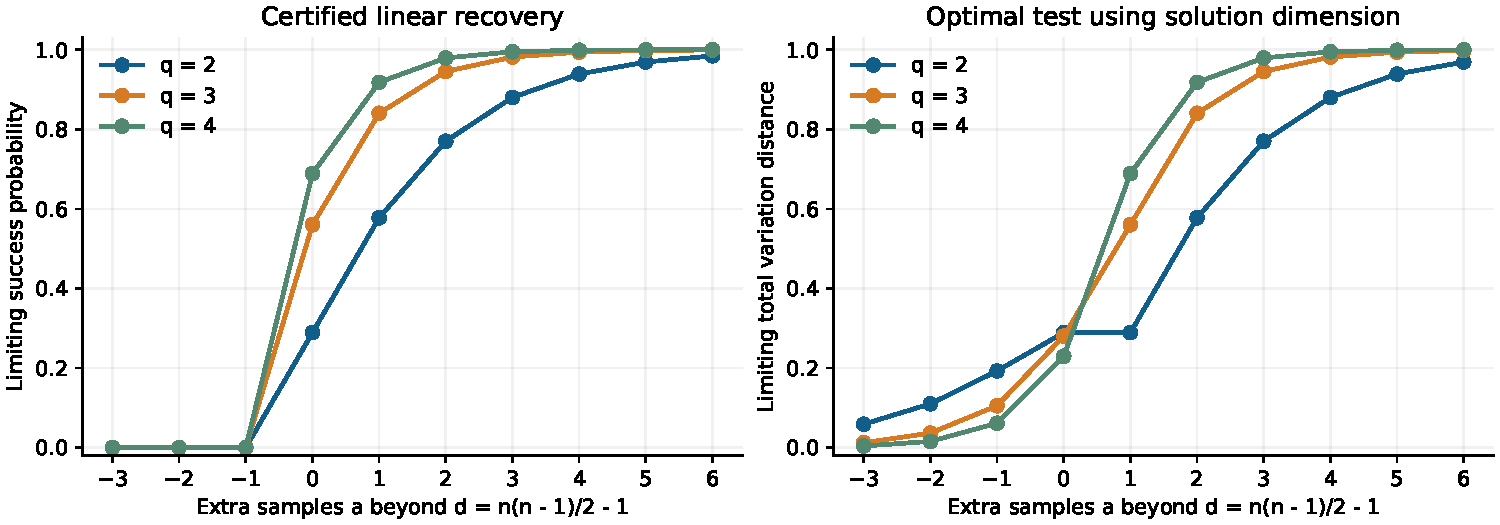
\includegraphics[width=\linewidth]{figures/critical_profiles.pdf}
\caption{Exact limiting profiles from Corollaries~\ref{crit:recovery} and~\ref{crit:testing}. The two panels concern different statistical tasks. The recovery algorithm certifies a one-dimensional solution space; the testing panel uses only its dimension.}
\label{fig:critical}
\end{figure}

\subsection{Independent exact checks}

The program \texttt{code/verify\_hidden\_forms.py} enumerates all two-planes and all alternating forms on $\mathbb F_2^4$ and $\mathbb F_3^4$. It computes incidences directly, separately from the theoretical Fourier formulas. There are respectively $35$ and $130$ two-planes, of which $15$ and $40$ are isotropic for the chosen nondegenerate form. The $64+729$ alternating forms give $2(64+729)=1586$ exact comparisons of the null and planted Fourier identities. All agree as rational numbers.

The same program computes complete finite-dimensional binary nullity laws by an exact dynamic program on row spaces, through $12$ observations for $n=4$. Its transition counts use the enumerated planes; it does not substitute the limiting iid law. These data provide small-dimensional examples, including a reminder that the asymptotic approximation need not be close when $n$ is small.

For numerical illustration, $5000$ independent trajectories in each of the null and planted models were generated at each of $n=6,10,14$, with seed $20261127$. The largest empirical distance from the limiting law over offsets $-2$ through $5$ was about $0.2032$ at $n=6$, $0.0124$ at $n=10$, and $0.0109$ at $n=14$. These are Monte Carlo comparisons containing both sampling error and finite-size effects; they are not proofs or deterministic error bounds. At the exact threshold $a=0$, the planted runs at $n=10$ gave $1435/5000=0.2870$ one-dimensional solution spaces, compared with the limit $0.2887880951\ldots$.

The products defining the plotted curves are truncated after $300$ factors. The elementary bound
\[
0\le1-\prod_{j>M}(1-q^{-j})\le\sum_{j>M}q^{-j}=\frac{q^{-M}}{q-1}
\]
controls this truncation. Standard double-precision rounding affects the printed last digits; the identities themselves are proved algebraically.

\subsection{The arithmetic decoder implementation}

The program \texttt{code/noisy\_path\_decoder.py} implements (NG4). It reads a real position array, the mesh, an optional position-error bound and a finite list of prime probes. Its default bandwidth is (NG11), with increment-error bound twice the supplied position-error bound. The chosen smooth window is
\[
w(v)=Z^{-1}\exp\!\left[-\frac1{(v-1)(2-v)}\right]\mathbf1_{(1,2)}(v),
\quad Z=\int_1^2\exp\!\left[-\frac1{(v-1)(2-v)}\right]dv,
\]
with $J_w\simeq1.96254112181544$. It reports the estimates, the asymptotic standard-deviation scale, and the two quantities in (NG9). It does not mislabel an asymptotic standard deviation as a finite-sample certified confidence interval.

The program \texttt{code/verify\_analytic\_algebra.py} checks the exact extrapolation identities for orders $1$ through $8$, including the allocation factor $(2^m-1)^2$. It also compares the decoder against a directly evaluated three-jump synthetic path to check the sign, angle inversion, and normalization. That synthetic path is not a Dirichlet Li--L\'evy path and supplies no empirical proof of the analytic theorem.

Floating-point evaluation is a practical illustration of the mathematical estimator. The theorem states separately how deterministic probe-evaluation errors enter the total error. A fully certified numerical implementation would need error-controlled transcendental evaluation and numerical upper bounds for the constants in (NG22). Neither is asserted by the included floating-point script.

\subsection{Rebuilding and the verification boundary}

The archive is self-contained for rebuilding the report. From its top directory run
\begin{verbatim}
pdflatex -interaction=nonstopmode -halt-on-error \
  finite_observation_and_critical_recovery.tex
pdflatex -interaction=nonstopmode -halt-on-error \
  finite_observation_and_critical_recovery.tex
python3 code/verify_hidden_forms.py --repetitions 5000
python3 code/verify_analytic_algebra.py
\end{verbatim}
The Python scripts use NumPy, SciPy and Matplotlib; their versions in the preparation environment are recorded in \texttt{results/environment.json}. The exact incidence checks and finite row-space enumeration use Python integers and rational arithmetic. JSON files retain the complete counts and numerical outputs.

The mathematical proofs were separately checked for source dependencies, generator-domain justification, adaptive-noise control, covariance scaling, low-rank exceptional sets, transition coupling, and stopping-time tails. The review corrected an initially proposed accelerated Gaussian assertion: the final higher-order theorem claims only the mean-square rates justified by its proof, while the sharp Gaussian theorem retains the narrower mesh conditions (NG9).

No new Lean proof is included. The artifact establishes its claims through the written proofs and supplemental finite checks. The upstream theorem's verification status is reported from its primary verification source, rather than inferred from these computations. Global novelty, growing-conductor statistical constants, the compatible nondegenerate-form count, and full-data optimal hidden-form testing remain outside the established conclusions.

\begin{thebibliography}{99}
\bibitem{ProveIt2026}
V. Reshetnikov, \emph{ProveIt: Generalized Riemann Hypothesis}, merged article and source files, pinned commit \texttt{7c24c5481fc0c8101b22b7e7cfab8321921c0faa}, 27 November 2026.
\href{https://github.com/VladimirReshetnikov/ProveIt/tree/7c24c5481fc0c8101b22b7e7cfab8321921c0faa/Analysis/GeneralizedRiemannHypothesis}{Pinned repository directory}.

\bibitem{Sutherland2026}
A. V. Sutherland, \emph{Verification files for the shorter Lean proof of RH and of GRH for Dirichlet $L$-functions}, page updated 27 November 2026, reporting checks of \texttt{lsernau/grh-lean} revision \texttt{72fead10}.
\url{https://math.mit.edu/~drew/shortgrh/}.

\bibitem{Figueroa2008}
J. E. Figueroa-L\'opez, Small-time moment asymptotics for L\'evy processes,
\emph{Statistics \& Probability Letters} \textbf{78} (2008), 3355--3365.
\href{https://doi.org/10.1016/j.spl.2008.07.012}{doi:10.1016/j.spl.2008.07.012}.

\bibitem{Nickl2016}
R. Nickl, M. Rei\ss, J. S\"ohl and M. Trabs, High-frequency Donsker theorems for L\'evy measures,
\emph{Probability Theory and Related Fields} \textbf{164} (2016), 61--108.
\href{https://doi.org/10.1007/s00440-014-0607-3}{doi:10.1007/s00440-014-0607-3};
\href{https://arxiv.org/abs/1310.2523}{arXiv:1310.2523}.

\bibitem{Gonzalez2021}
J. Gonz\'alez C\'azares and J. Ivanovs, Recovering Brownian and jump parts from high-frequency observations of a L\'evy process,
\emph{Bernoulli} \textbf{27}(4) (2021), 2413--2436.
\href{https://doi.org/10.3150/20-BEJ1314}{doi:10.3150/20-BEJ1314};
\href{https://arxiv.org/abs/2003.05363}{arXiv:2003.05363}.

\bibitem{FulmanGoldstein2015}
J. Fulman and L. Goldstein, Stein's method and the rank distribution of random matrices over finite fields,
\emph{Annals of Probability} \textbf{43}(3) (2015), 1274--1314.
\href{https://doi.org/10.1214/13-AOP889}{doi:10.1214/13-AOP889};
\href{https://arxiv.org/abs/1211.0504}{arXiv:1211.0504}.

\bibitem{Cascudo2015}
I. Cascudo, R. Cramer, D. Mirandola and G. Z\'emor, Squares of random linear codes,
\emph{IEEE Transactions on Information Theory} \textbf{61}(3) (2015), 1159--1173.
\href{https://doi.org/10.1109/TIT.2015.2393251}{doi:10.1109/TIT.2015.2393251};
\href{https://arxiv.org/abs/1407.0848}{arXiv:1407.0848}.

\bibitem{Randriambololona2015}
H. Randriambololona, \emph{Linear independence of rank 1 matrices and the dimension of $*$-products of codes}, 2015.
\href{https://arxiv.org/abs/1501.05978}{arXiv:1501.05978}.
\end{thebibliography}

\end{document}
